\documentclass{article}
\usepackage{url,graphicx,color}

\newcommand{\BEASTVersion}{2.4.1}
\newcommand{\TracerVersion}{1.6}
\newcommand{\FigTreeVersion}{1.4.2}


\def\beast-geo{GEO\_SPHERE}
\def\lt{\textless}
\def\gt{\textgreater}


\begin{document}
\title{Advanced Phylogeography with BEAST \BEASTVersion\\
    {\small Somewhat Inhomogeneous phylogeography, tip sampling, geographical priors}}
\author{Remco Bouckaert \url{r.bouckaert@auckland.ac.nz}}
\maketitle

\section{Introduction}


In this tutorial we describe how to set up an analysis using inhomogeneous diffusion as described in  \cite{somewhatIP} with the full Bayesian framework for phylogeography \cite{sphericalgeo}. It is assumed that you have done other tutorials (especially the 'Continuous phylogeography on a sphere' tutorial) and know how to run BEAST, Tracer, SPREAD and create a heatmap using the HeatMapMaker app, as outlined in the 'Continuous phylogeography on a sphere' tutorial.

Somewhat heterogeneous diffusion can be achieved by transforming the Mercator projection, thus getting a new map where the standard diffusion process is run. The transformation can be based on a cartogram, where the area is transformed such that higher density shapes are blown up and lower density ones are shrunk. The image above shows the standard Mercator projection world map left and a cartogram where country sizes represent population sizes on the right. To use a cartogram transformation, create a file containing shapes in ESRI shape file or KML file. ESRI shape files allow attributes to be associated directly with shapes, which can be used as density or weight. For KML files, each shape has a name, and in the BEAST XML you can specify for each of these names the weight it should get.

{\bf Note}: The deformation grid that is generated only covers the bounding box around the shapes, to the shapes should be covering the area of interest. You can place dummy shapes at the corners in order to ensure the bounding box is big enough.

You will need the following software at your disposal:

\begin{itemize}

\item {\bf BEAST} - This package contains the BEAST program, BEAUti, TreeAnnotator and other utility programs. This tutorial is written for BEAST v{\BEASTVersion}\footnote{It will not work as smooth with BEAST v2.4.0.}. It is available for download from \\* \texttt{http://beast2.org/}.
\item {\bf Tracer} - this program is used to explore the output of BEAST (and other Bayesian MCMC programs). It graphically and
quantitively summarises the distributions of continuous parameters and provides diagnostic information. At the time of
writing, the current version is v{\TracerVersion}. It is available for download from \texttt{http://beast.bio.ed.ac.uk/}.i
\item {\bf Spread} for summarising the geographic spread in a KML file (available from \url{http://www.kuleuven.ac.be/aidslab/phylogeography/SPREAD.html}.
\item {\bf google-earth} for displaying the KML file (just google for it, if you have not already have it installed).
\end{itemize}


This tutorial guides you through a continuous phylogegraphy analysis of a new tree based on Indo-European languages and we will examine the impact of a reduced migration through the Caucasus by decreasing the rate of migration through that area. Note that you can co-estimate the tree and geography, so it is not a requirement to fix the tree, but for the tutorial fixing the tree makes it practical to perform a substantial analysis in a short amount of time.

We go through the following steps:
\begin{itemize}
\item The first step is to install the \beast-geo{} package that contains the phylogegraphic model. 
\item Then, we use BEAUti to set up the analysis, and write it to an XML file.
\item We use BEAST to run the MCMC analysis based on the XML file.
\item The results will need to be checked for convergence using Tracer.
\item Finally, we post-process the output of the MCMC so we can visualise the geographical dispersion.
\end{itemize}

\subsection*{Install \beast-geo\ package}

Phylogeography as described in this tutorial is part of the {\tt \beast-geo} package.

If you not already have it installed, you can install the package through BEAUti. Start BEAUti by double clicking on its icon. 
Select the File/Manage packages menu. A dialog pops up showing the packages already installed. 

{\bf Note:} if you already had the package installed, make sure you upgrade to the latest version.

\begin{center}
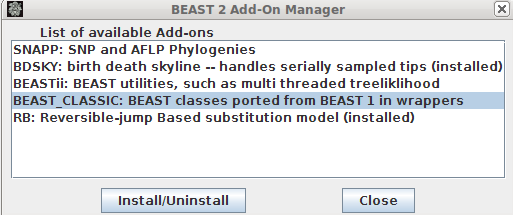
\includegraphics[scale=0.4]{figures/addonmgr.png}
\end{center}

Select the \beast-geo{} entry in the list, and click the Install button. After a little while the dialog is updated and it shows that the package is now installed. The BEASTLabs package will automatically be installed as well, since \beast-geo{} depends on this package.

\subsection*{BEAUti}

Select the menu ``File/Set working dir/\beast-geo" since we are going to work with files from the beast-geo package (you may need to restart BEAUti if you just installed the package).

\begin{center}
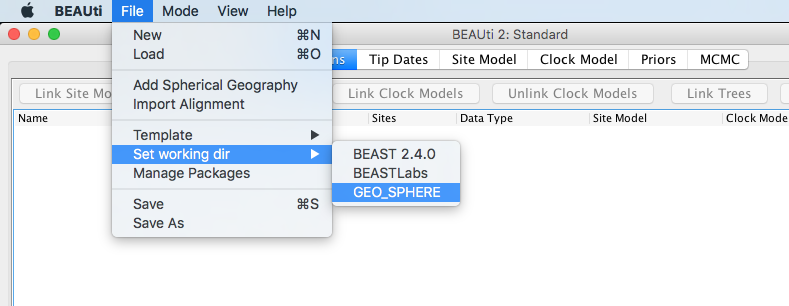
\includegraphics[scale=0.4]{figures/BEAUti_setWD}
\end{center}

Select the ``File/Add Spherical Geography" menu item  and a dialog pops up that asks for a trait name and a tree. Use 'geo' for trait name and Since we will use a fixed tree, leave the selection on '[[fixed tree]]'.

\begin{center}
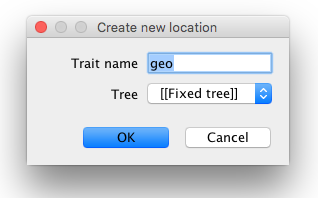
\includegraphics[scale=0.4]{figures/BEAUti_transform1}
\end{center}

A file selection dialog pops up. Select the file ``examples/transform/IE.tree" from the beast-geo folder. The file IE.tree contains a tree in NEXUS format. Now, a dialog pops up with a table of locations and a list of languages from the tree.

\begin{center}
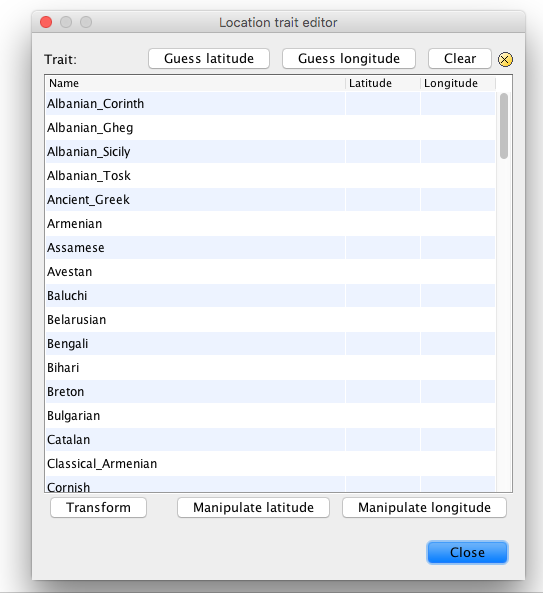
\includegraphics[scale=0.4]{figures/BEAUti_transform2}
\end{center}

You can fill in the individual entries by hand, but if you press the 'Guess latitude' button, a dialog pops up that helps you fill these entries.
The easiest way to populate the table is by importing it from a file containing the table in comma separated format. Select the 'read from file' option and click 'browse'. Select the file 'examples/transform/IElocations.dat' in the beast-geo package folder.

\begin{center}
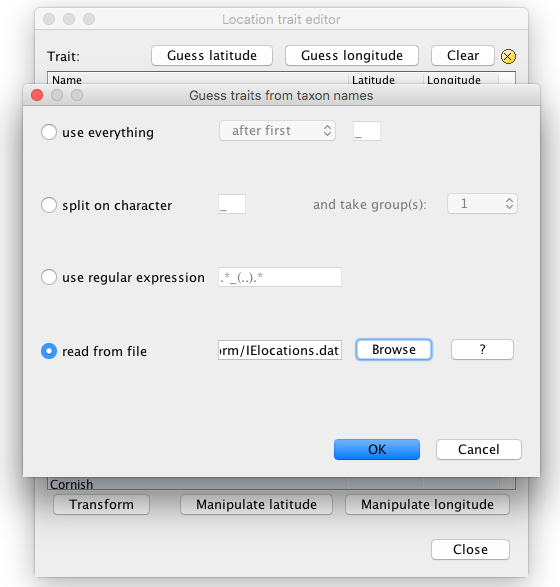
\includegraphics[scale=0.4]{figures/BEAUti_transform3}
\end{center}

After clicking OK, the table with locations will be populated and look something like this:

\begin{center}
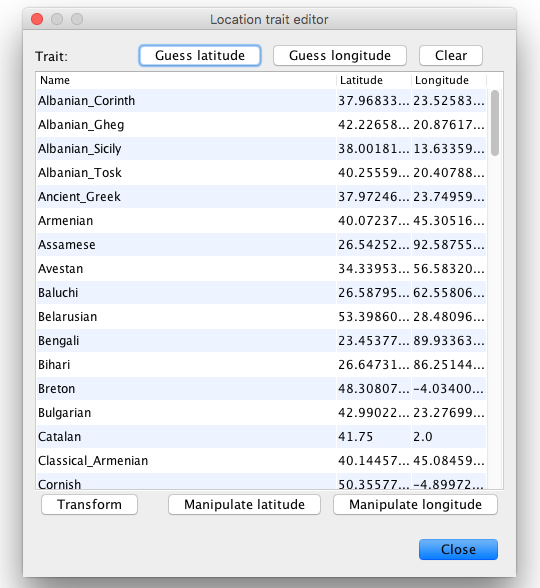
\includegraphics[scale=0.4]{figures/BEAUti_transform4}
\end{center}

Click 'Close' and you have created a partition called IE that is shown in the partition panel. Now we can set up the clock model by switching to the clock model panel. By default, a relaxed clock is assumed, but for this data a relaxed log normal fits much better, so select this model from the drop down box. The 'estimate' box for the clock rate will be greyed out, but since we want to estimate the rate, select the menu 'Mode/Automatically set clock rate' and make sure it is not checked. 

\begin{center}
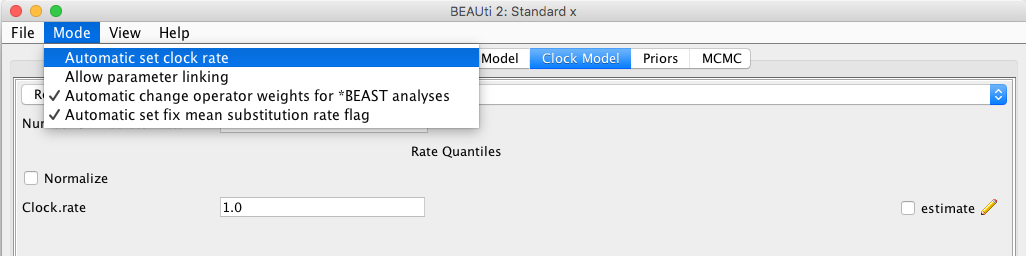
\includegraphics[scale=0.4]{figures/BEAUti_transform5}
\end{center}

The estimate box now can be checked.

\begin{center}
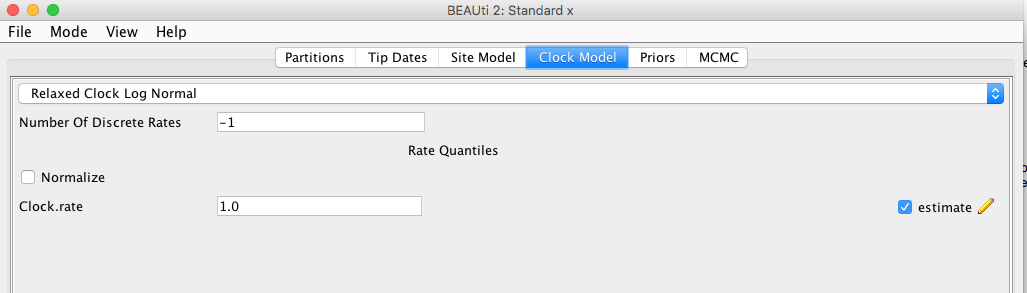
\includegraphics[scale=0.4]{figures/BEAUti_transform6}
\end{center}

We do not wan the standard deviation for the relaxed clock to get out of hand, so set an alarm limit of 5 on it. Select the menu ``View/Show Initialisation Panel" and set the upper field to 5;

\begin{center}
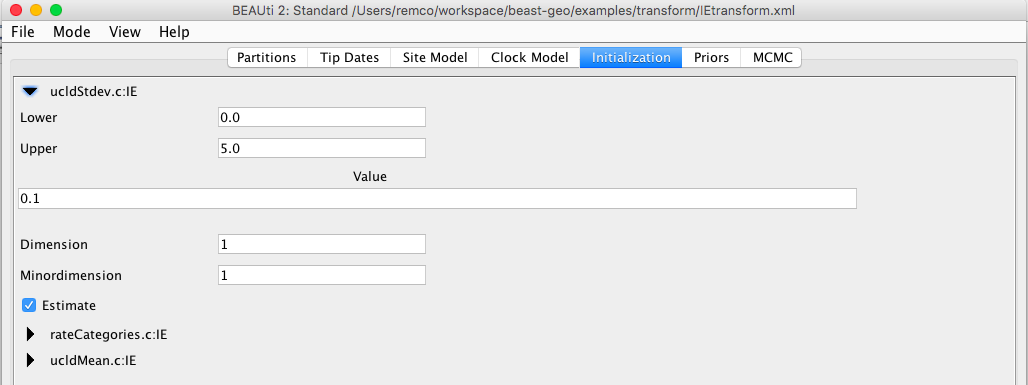
\includegraphics[scale=0.4]{figures/BEAUti_transform7} 
\end{center}

In the MCMC panel, set the chain length to 1 million, and set logging frequency for trees to 10000. Save the file as a IE.xml using the ``File/Save" menu. Now you can run the file in BEAST, check convergence in Tracer (for 1 million, it does not convergence, so ESSs are poor, but for the purpose of this tutorial it gives a good indication of the geography. You can resume for another million states or more to get full convergence.) To visualise the result using {\tt spread} create a summary tree from a terminal using
\begin{verbatim}
/path/to/treeannotator -hpd2D 0.8 -b 10 IE.trees > IE.tree
\end{verbatim}
This creates 80\% HPD areas in the annotated tree. Do not forget the -hpd2D argument, otherwise no HPD regions will be shown. 
In {\tt spread}, go to the continuous tab, select IE.tree as tree, and select 'location1' and 'location2' for 'latitude attribute name' and 'longitude attribute name' respectively. Then under the 'output' tab, click 'Plot' to visualise in {\tt spread}, or 'Generate' to generate a KML file that can be shown in Google earth. See the spherical geography tutorial for details.


\section*{Inhomogeneous phylogeography}

Now we are going to add a transformation to the analysis. In BEAUti, go to the partitions panel, and double click the IE entry on say the file. The table editor for locations pops up again, where you click the ``Transform" button.

\begin{center}
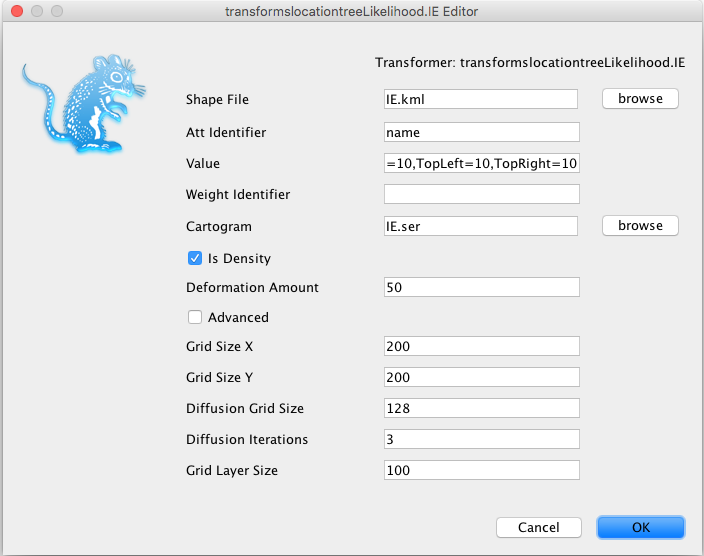
\includegraphics[scale=0.4]{figures/BEAUti_transform8}
\end{center}

A shape file or KML file can be used as input to the cartogram. KML files can easily be prepared in Google Earth and other software and shape files are the standard format for most GIS programs. We will use a KML file that has 1 area representing the Caucasus, and three dummy elements -- these are required since the cartogram transforms space increasing areas relative to other areas. If there is no other area specified, the transformation will be a uniform one. Here they are shown in red for the Caucasus and green for the three dummy areas;

\begin{center}
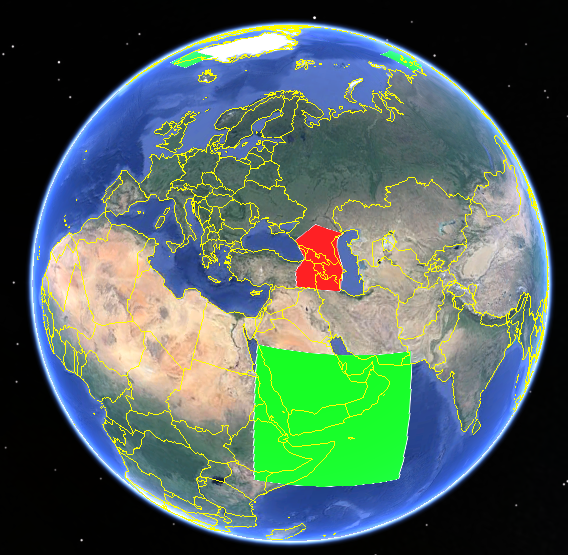
\includegraphics[scale=0.4]{figures/IEmap.png}
\end{center}

Select examples/transform/IE.kml in the \beast-geo{} folder for the shape file by clicking the ``browse" button next to the ``Shape file" entry.

Each of the areas has a name; Caucasus, Dummy, TopLeft and TopRight. To set the relative weights for each of the different areas, fill in\\ ``Caucasus=1000,Dummy=10,TopLeft=10,TopRight=10" in the entry for ``value". 

If you specify the file for the Cartogram entry, the cartogram (which can take a bit of time to be calculated) is saved in that file, and next time BEAST will attempt to read that file first, so the cartogram does not have to be recalculated. Of course, this means when changing the shape file that you have to remove the cartogram file, otherwise the analysis will run with the old shape file.

You want to make sure that the path of the cartogram entry exists, otherwise no file will be written. 

The transfomer has the following general attributes:\\

{\tt shapeFile}: file containing regions in .shp or .kml format. Must be specified.\\

{\tt attIdentifier}: name of attribute in shape file that identifies a region, default ``NAME".\\

{\tt value}: comma separated list of 'id=value' pairs where values representing relative size for each regions with ID from the shape file.\\

{\tt weightIdentifier}: name of attribute in shape file that identifies a weight, either specify weightIdentifier or value, but no both.\\

{\tt isDensity}: if true, weights are interpreted as densities, otherwise they are interpreted as mass, default true.\\

{\tt cartogram}: File containing cartogram. If specified and file does not exist, the cartogram will be calculated and stored there so that on resuming a run the cartogram does not need to be recalculated.\\

{\bf Note:} to govern the behaviour of the transformation, there is a simple option (when {\tt advanced=false}) where the deformation amount is specified and all other parameters are estimated, or each of the parameters can be specified individually (when {\tt advanced=true}).\\

{\tt advanced}: if true the advanced parameters should be taken in account, otherwise these are estimated. Default false.\\

{\tt deformationAmount}: Defines the amount of deformation. This is an integer value between 0 and 100. The default value is 50. Ignored if advanced=true.\\

{\tt gridSizeX}: A first grid is applied to the main transformation layer. 
This rectangular grid is defined by the number of columns. 
Higher numbers produce denser grids and thus a better cartogram quality. 
However, a denser grid also implies a longer treatment. 
Default 200, ignored if advanced=false.\\

{\tt gridSizeY}: As gridSizeX but for number of rows, default 200, ignored if advanced=false\\

{\tt diffusionGridSize}: A second grid is applied to the main transformation layer. 
This square grid is defined by the number of rows. 
Denser grids imply again a better cartogram quality but longer computation times.
must be a power of 2, default 128, ignored if advanced=false.\\

{\tt diffusionIterations}: The second grid is transformed with the Gastner/Newman diffusion 
algorithm, which can be run several times to obtain a higher transformation quality. 
Higher numbers of iterations also imply longer treatment times.
Default 3, ignored if advanced=false.\\

{\tt gridLayerSize}: The visualisation grid layer size. After starting the BEAST run, two files are produced:
{\tt scapetoad.svg} containing the deformation grid and original shapes but transformed, and 
{\tt deformationLayer.svg} which contains only the deformation grid. These can be used to see whether the transformation is somewhat reasonable. This is the gridsize which is produced for visual effect only in the sag files. 
Default 100.


Go to the MCMC panel, and set the tracelog file name to IEtransformed.log, and the tree log file name to IEtransformed.trees, and make sure the log frequency is set to once very 10 thousand.
\begin{center}
\includegraphics[scale=0.4]{figures/BEAUti_transform20}
\end{center}

{\bf Note:} do not use File/Save, since it will overwrite the file IE.xml saved earlier. Save the file as a IEtransform.xml using the ``File/Save as" menu.

\subsection*{Running BEAST and analysing the output}

Running BEAST and analysing the results on the two files is similar as the phylogeography tutorial. Use tracer to check convergence, and use spread with Google Earth and/or the HeatMapMaker application via the BEAST AppStore to visualise the geographical history over the tree. For details, refer to the phylogeography tutorial.

When running BEAST, two SVG files are written: toadmap.svg avd deformationLayer.svg. These contains information of the transformed map, the toadmap contains the regions, and the deformation layer only the transformed grid, and look like this:

\includegraphics[width=0.5\textwidth]{figures/deformationlayer.pdf}
\includegraphics[width=0.5\textwidth]{figures/toadmap.pdf}

After running the analysis in BEAST, check the log file in Tracer (again, 1 million states is not sufficient to get to convergence. You can run for longer if you like to get full convergence by resuming the run.).

To create a heatmap, open the BEAST AppStore and launch the HeatMapMaker. In the dialog that pops up, select IEtransformed.trees for tree set, set bounding box to -20 -30 70 120, set tag to 'location', height to 512,  and click OK. A heatmap png and /tmp/legend.png (which shows colours associated with some time in the past) file will be generated that looks something like this.

\includegraphics[width=0.75\textwidth]{figures/IEheatmap}
\includegraphics[width=0.25\textwidth]{figures/IElegend}

Do these differ much from the non-transformed analysis?

\section*{Advanced geographical analyses by editing the XML}
\subsection*{Adding a transformer}
To add a transformer by editing the XML instead of BEAUti you do the following: Once the shape file is created, add the following element to the {\tt sphericalGeo.ApproxMultivariateTraitLikelihood}. If you have information in a shape file, add something like

\begin{verbatim}
 <transformer id="transformer" 
       shapeFile="TM_WORLD_BORDERS_SIMPL-0.3.shp" 
       attIdentifier="NAME" 
       weightIdentifier="POP2005" 
       spec="sphericalGeo.scapetoad.ScapeToadTransfomer"
       cartogram="cartogram-population.ser"/> 
 \end{verbatim}

If you have information in a KML file, add something like

\begin{verbatim}
<transformer id="transformer" shapeFile="IE.kml"
      attIdentifier="name"
      value="Caucasus=1000,Dummy=10,TopLeft=10,TopRight=10"
      spec="sphericalGeo.scapetoad.ScapeToadTransfomer"
      cartogram="cartogram-population2.ser"/>
\end{verbatim}

\subsubsection*{Sampling tip locations}
At this point in time, there is no BEAUti support to allow sampling of tip locations, but it can be done by editing the XML once it is produced by BEAUti.

First, you need to add an entry to the state, and add operators.
Second, you have to define a set of regions, either by KML or by colouring a bitmap image in Mercatore projection. KML regions can be drawn in google-earth and bitmap images in Mercator projection can be produced using the MapMaker utility that you can start from the BEAST AppStore. Once you created a world map with MapMaker, you can colour in the region you want to sample from.

To set up the state, add the following line (where ``geo" is the name used for the geography partition)

\begin{verbatim}
<stateNode idref="location.s:geo"/>
\end{verbatim}

Note that the ``s:" in ``location.s:geo" is important!
Next, add a LocationOperator to the set of operators (inside the MCMC element, where the other operators are):

\begin{verbatim}
<operator id='location.sampler' spec='sphericalGeo.LocationOperator' 
    location='@location.s:geo' 
    likelihood='@slocationtreeLikelihood.geo' weight='30'/>
\end{verbatim}

Also, add a reference to {\tt location.s:geo} in ApproxMultivariateTraitLikelihood by adding the attribute {\tt location="@location.s:geo"} to the element with {\tt id="slocationtreeLikelihood.geo"}.

To specify a KML region, add the following fragment to the XML at the top level (just under the alignment, but above the run element would be a good place).

\begin{verbatim}
<region id='China' spec='sphericalGeo.region.KMLRegion' kml='kml/China.kml'/>
\end{verbatim}

This creates a KMLRegion with id China, and reads in the kml file in the folder kml from file China.kml. To create a bitmap region from a bitmap file stored in say regions/China.png, you can use

\begin{verbatim}
<region id='China' spec='sphericalGeo.region.BitMapRegion'
	file='regions/China.png'/>
\end{verbatim}
There is an extra option to specify a bounding box by two latitude/longitude pairs if the bitmap only covers a small region of the map instead of the whole world:
\begin{verbatim}
<region id='China' spec='sphericalGeo.region.BitMapRegion'
	file='regions/China.png' bbox=''/>
\end{verbatim}



Now we defined a region, suppose you want to sample taxon AF182802 from the region of China, you add

\begin{verbatim}
<geoprior location='@location.s:geo' tree='@Tree.t:hbv' region='@China'
	spec='sphericalGeo.GeoPrior'>
	<taxon id='AF182802' spec='Taxon'/> 
<geoprior>
\end{verbatim}

inside the element with id='slocationtreeLikelihood.geo' (where 'geo' is the name of the partition for spherical geography, and `hbv' the name of the partition with the alignment).


If you have many regions and tips you want to sample, to prettify the XML and make it somewhat more readable, you can create these maps:

\begin{verbatim}
<map name="region">sphericalGeo.region.KMLRegion</map>
<map name="geoprior">sphericalGeo.GeoPrior</map>
\end{verbatim}

and then you can leave out the spec attribute and instead of the above use

\begin{verbatim}
<region id='China' kml='kml/China.kml'/>
\end{verbatim}

and 

\begin{verbatim}
<geoprior location='@location.s:geo' tree='@Tree.t:hbv' region='@China'>
	<taxon id='AF182802' spec='Taxon'/>
<geoprior>
\end{verbatim}



Finally, in order to initialise the locations and let the likelihood know which locations are sampled, and which are approximated directly, we have to do two things:\\
1. let the {\tt ApproxMultivariateTraitLikelihood} know where the location parameter is by adding the location-attribute, and\\
2. add an entry for every {\tt geoprior}.

After this, the XML for the geography likelihood should look something like this:

\begin{verbatim}
      <distribution id="geography" spec="sphericalGeo.ApproxMultivariateTraitLikelihood" tree="@Tree.t:AFRICA" 
		location idref="location.s:geo">
        <geoprior idref="China"/>
        <geoprior idref="Eurasia"/>
        ...
\end{verbatim}


\subsubsection*{Putting a prior on the root locations}

Putting a prior on the root means we have to sample the root location, which essentially follows the recipe for sampling tips, but instead of specifying a single taxon, we specify a taxon set containing all taxa. If we want to restrict the root location to China, as specified above, this can be done for example like so:

\begin{verbatim}
<geoprior location='@location.s:geo' tree='@Tree.t:hbv' region='@China'>
	<taxonset id='all.taxa' spec='TaxonSet' alignment='@hbv'/>
<geoprior>
\end{verbatim}


\subsubsection*{Putting a prior on a monophyletic clade}

First, specify a monophyletic clade in the priors panel in BEAUti; hit the little '+' button at the bottom, and a dialog pops up where you can specify a taxon set. Once you have given the clade a name (say ``myclade") and close the dialog, in the priors panel a new entry appears for the clade. Select the 'monophyletic' check box. Note that the clade must be monophyletic, otherwise the sampler does not work.

To specify the prior, add the following to the element with {\tt id="slocationtreeLikelihood.geo"}

\begin{verbatim}
<geoprior location='@location.s:geo' tree='@Tree.t:hbv' region='@China'>
	<taxonset idref='myclade'/>
<geoprior>
\end{verbatim}




\bibliographystyle{plain}

\bibliography{phylogeography_s}


\end{document}
